\documentclass{ieeeaccess}
\usepackage{cite}
\usepackage{amsmath,amssymb,amsfonts}
\usepackage{algorithmic}
\usepackage{graphicx}
\usepackage{textcomp}


\usepackage{hyperref}
\usepackage{mathtools}

\usepackage{lipsum}
\usepackage{bm}
\makeatletter
\AtBeginDocument{\DeclareMathVersion{bold}
\SetSymbolFont{operators}{bold}{T1}{times}{b}{n}
\SetSymbolFont{NewLetters}{bold}{T1}{times}{b}{it}
\SetMathAlphabet{\mathrm}{bold}{T1}{times}{b}{n}
\SetMathAlphabet{\mathit}{bold}{T1}{times}{b}{it}
\SetMathAlphabet{\mathbf}{bold}{T1}{times}{b}{n}
\SetMathAlphabet{\mathtt}{bold}{OT1}{pcr}{b}{n}
\SetSymbolFont{symbols}{bold}{OMS}{cmsy}{b}{n}
\renewcommand\boldmath{\@nomath\boldmath\mathversion{bold}}}
\makeatother

\def\BibTeX{{\rm B\kern-.05em{\sc i\kern-.025em b}\kern-.08em
    T\kern-.1667em\lower.7ex\hbox{E}\kern-.125emX}}

\newcommand{\Tau}{\scalebox{1.60}{$\tau$}}
% For generic tf's
% \newcommand{\tf}[2]{\prescript{#1}{}{T_{#2}}}
\newcommand{\tf}[2]{\prescript{#1}{}{\mathbf{T}^{#2}}}
\newcommand{\tfC}[3]{\prescript{#1}{}{\mathbf{T}^{#2}_{#3}}}
\newcommand{\tfEstimated}[2]{\prescript{#1}{}{\mathbf{\hat{T}}^{#2}}}
\newcommand{\tfEstimatedC}[3]{\prescript{#1}{}{\mathbf{\hat{T}}^{#2}_{#3}}}

% For atomic tf's
\newcommand{\tfAtomic}[2]{\prescript{#1}{}{\mathbf{\Tau}^{#2}}}
\newcommand{\tfAtomicC}[3]{\prescript{#1}{}{\mathbf{\Tau}^{#2}_{#3}}}

% For atomic estimated tf's
\newcommand{\tfAtomicEstimated}[2]{\prescript{#1}{}{\mathbf{\hat{\Tau}}^{#2}}}



\newcommand{\optParam}[2]{\prescript{}{#1}{\mathbf{\hat{\Tau}}_{#2}}}

%
\newcommand{\intrisics}[1]{\mathbf{K}_{#1}}

% Maybe unnecessary but makes sure I dont screw up
\newcommand{\coordsthreeD}[2]{\mathbf{#1}_{#2}}
\newcommand{\coordstwoD}[2]{{#1}_{#2}}

\newcommand{\rotationComponent}[3]{\prescript{#1}{}{\mathbf{R}^{#2}_{#3}}}
\newcommand{\translationComponent}[3]{\prescript{#1}{}{\mathbf{t}^{#2}_{#3}}}

%Your document starts from here ___________________________________________________
\begin{document}
% \history{Date of publication xxxx 00, 0000, date of current version xxxx 00, 0000.}
% \doi{10.1109/ACCESS.2024.0429000}

\title{Annotation of Calibration Patterns for RGB-LiDAR Evaluations using Segmentation Models}
\author{\uppercase{Bruno Silva}\authorrefmark{1},PhD. Student\\
\uppercase{Gonçalo Ribeiro}\authorrefmark{1},PhD. Student}

\address[1]{Department of Mechanical Engineering, University of Aveiro}
% \address[2]{Department of Physics, Colorado State University, Fort Collins,
% CO 80523 USA (e-mail: author@lamar.colostate.edu)}
% \address[3]{Electrical Engineering Department, University of Colorado, Boulder, CO
% 80309 USA}

% \markboth
% {Author \headeretal: Preparation of Papers for IEEE TRANSACTIONS and JOURNALS}
% {Author \headeretal: Preparation of Papers for IEEE TRANSACTIONS and JOURNALS}


\begin{abstract}

  Extrinsic calibration is a crucial step in sensor fusion. This work presents a deep-learning-based augmentation to ATOM, a
  multi-sensor and multi-modal calibration framework, for automating the annotation of the outer borders of calibration patterns,
  eliminating the need for manual labeling. Instead of predicting the outer corners directly with a CNN/FC combo, which proved
  infeasible due to variable output sizes, we trained segmentation models to detect the pattern and later extracted the edges using
classical computer vision techniques. After testing various architectures, a U-Net model with a pretrained ResNet50 backbone delivered
the best results. \end{abstract}

\begin{keywords}
Extrinsic Calibration, Robot Calibration, Calibration Pattern, Machine Learning
\end{keywords}

\titlepgskip=-21pt

\maketitle

\section{Introduction}
\label{sec:introduction}

Extrinsic calibration is a fundamental process in robotics vision that involves determining the
relative pose (position and orientation) between different sensors, known as \textit{sensor to sensor calibration}, or between a sensor and a known reference
frame, which is known as \textit{sensor to coordinate frame}. Extrinsic calibration is crucial because it allows for the accurate integration of data from multiple sensors,
enabling sensor fusion. For instance, in an autonomous vehicle, the visual information of the camera
needs to be accurately aligned with the distance measurements of the LiDAR to build a coherent understanding of the
surroundings. Similarly, in robot arms, the position of the camera position relative to the end-effector must be precisely
known to perform tasks like object manipulation~\cite{atom}. 

Usually, iterative approaches are used. These rely on a cost function specific to a sensor modality but usually suffer from ambiguities
in some way or another. An typical cost function for an RGB camera relies on computing the difference between the projection of the
detection in the 2D image of some key points into a coordinate frame where these key points are precisely known. The objects that
contain these precisely known points are called \textit{Calibration patterns}. The most common types are chessboards and \textit{ChArUcos}.
\textit{ChArUcos} are chessboards with unique identifiable symbols embedded on each square that allow computer vision algorithms to decipher if the
pattern is upside down or if the framing of the image cuts part of the calibration object off. The issue with the aforementioned RGB cost function is that they
have multiple local minima and not always converge. A simple example is to picture an RGB camera fixed on the end of a prismatic joint
with the calibration pattern in front of the sensor, perfectly perpendicular to it. Both moving the offset of the joint or
moving the RGB sensor on the mount can lead to the same relative distance between the sensor and
the pattern, leading to equal detections of the key points, thus leading to
ambiguity~\cite{atom}. 

Despite the shortcomings mentioned, these cost functions have the advantage of generally performing more accurately in larger systems,
as there is much more variety of data, and can still be used effectively in most simpler systems, as their requirements are only the
existence of a sensor and a pattern. However, this creates the need for true evaluation procedures to assess the quality of the
calibration results and to make them comparable in order to be publishable~\cite{atom}. 

This project tackles an improvement to a previously fully manual and cumbersome evaluation method between RGB and LiDAR sensors,
integrated on ATOM~\cite{atom}, a well established multi-sensor multi-modal calibration framework in the
scientific community. The working principle is that by knowing the
physical outer limits of the pattern in the 2D image, these points can be projected into the coordinate frame of LiDAR sensor, provided
that the camera intrinsics are known. Afterward, the 3D points resulting from the projection can be directly compared with the 3D
points of the outer border of the pattern. This comparison is not ambiguous as the projected points only line up in the 3D frame if the
geometric transformations required for the projection are indeed correct. In ATOM, the 3D border points are already priorly labeled as
they are a requirement for the cost function that optimizes the pose of the 3D LiDAR sensors. However, the 2D points of the border are not
required by the RGB cost function. The current solution is a manual border labeling method, as a
simple automatic method would struggle with detecting orientation and deal with edge cases.~\cite{camera_lidar} This
project aims to develop an automatic method using deep learning to simplify the evaluation pipeline to the user. \autoref{fig:input}
and \autoref{fig:output} represent an example input and a desired output. On the output, each color encodes the border of one of the
sides of the calibration pattern.

\begin{figure}[h]
    \centering
    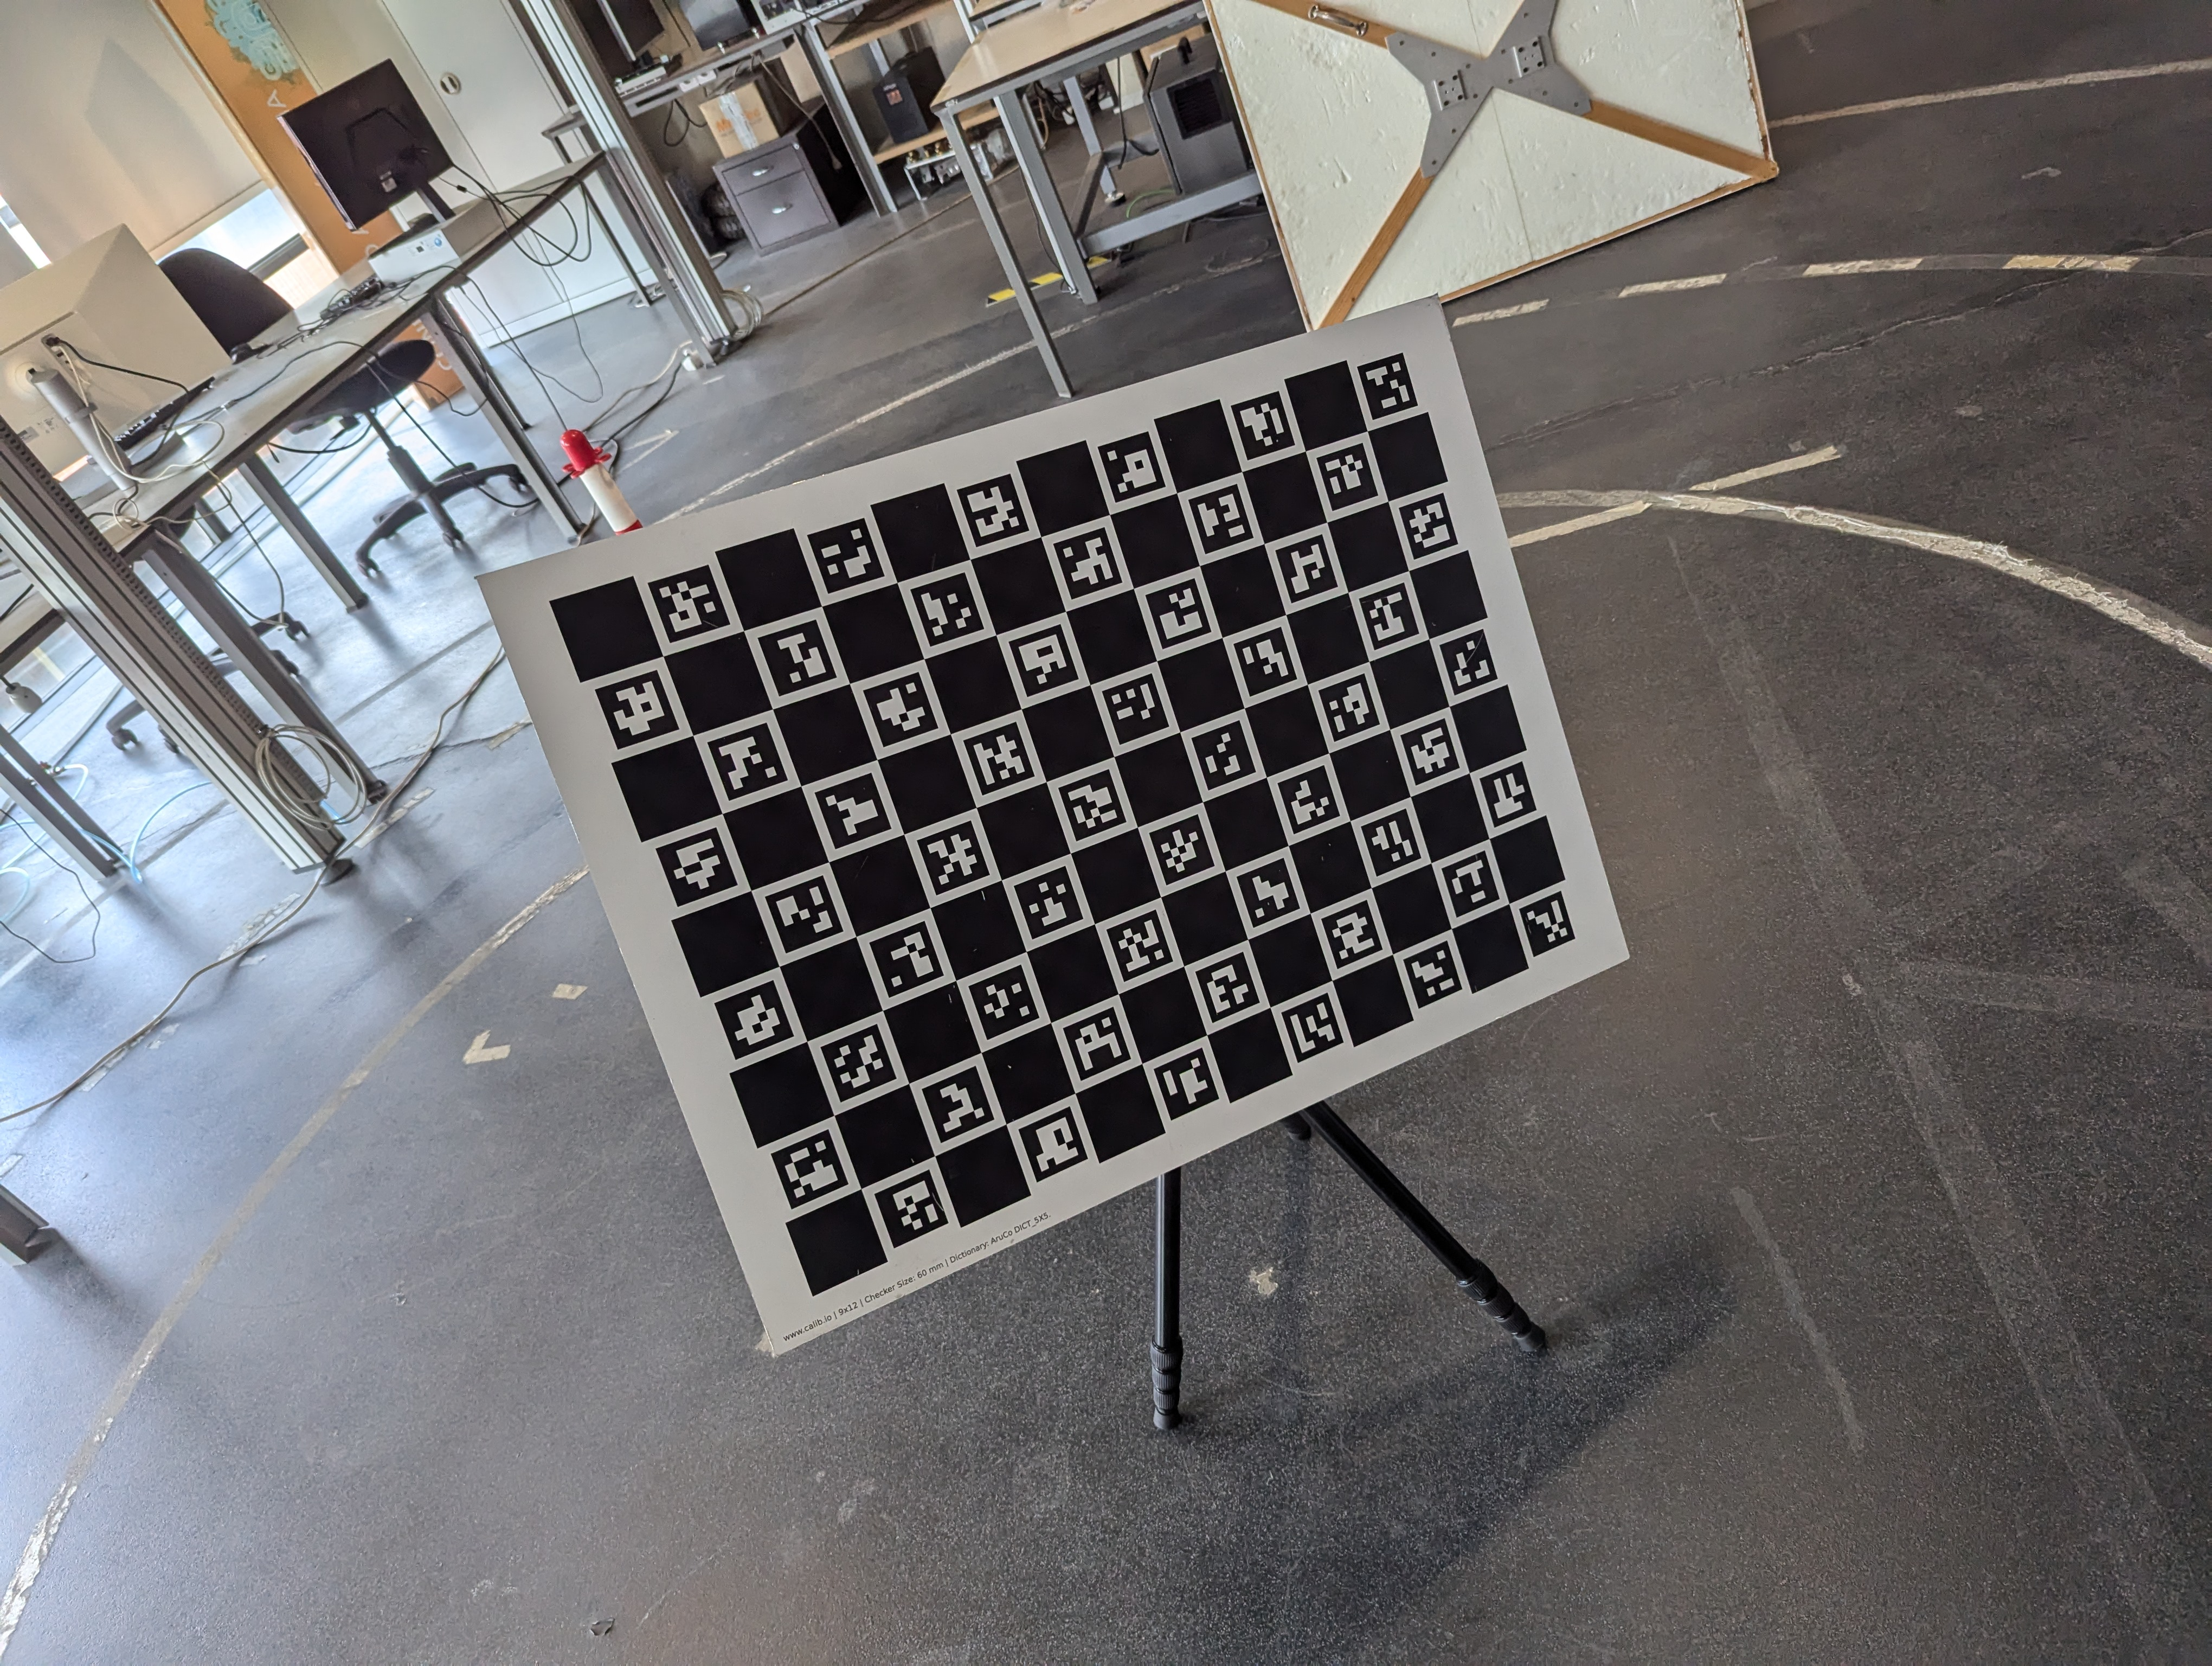
\includegraphics[width=0.8\linewidth]{resources/images/pattern_28.jpg}
    \caption{Example of an input image for the automatic labeler we aim to develop.}
    \label{fig:input}
\end{figure}

\begin{figure}[h]
    \centering
    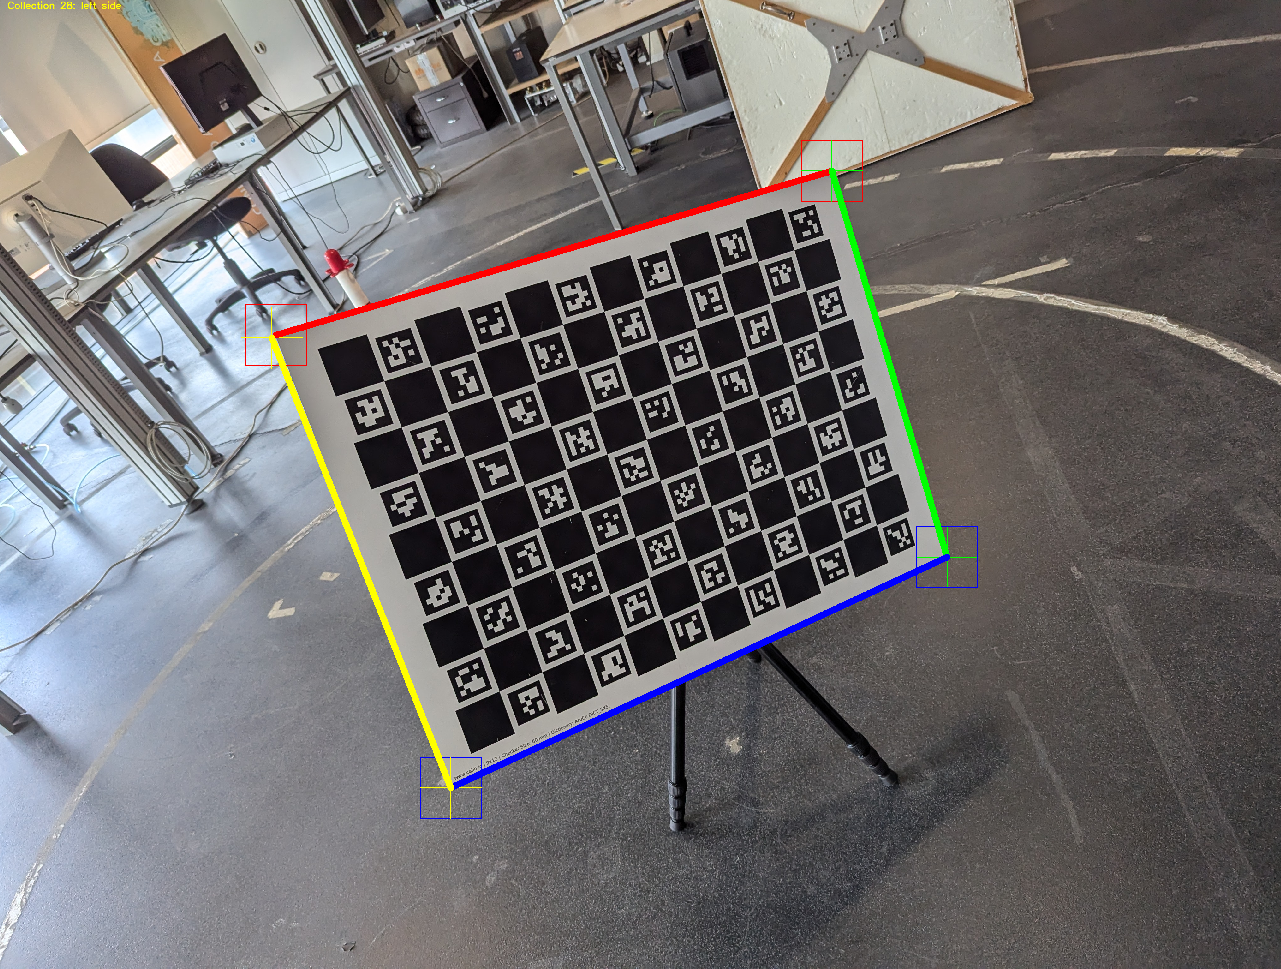
\includegraphics[width=0.8\linewidth]{resources/images/pattern_28_lines.png}
    \caption{Expected output from the automatic labeler, where the top border is marked in red, the right border in green, the bottom border in blue, and the left border in yellow.}
    \label{fig:output}
\end{figure}


\section{Proposed Approach}
\subsection{Data preparation}

% The data we had:
%   -  Images with corners labeled
%
% Captured more images to have more dataset diversity with other types of calibration patterns
%
% Developed a annotation program to label corners of the patterns. 
% Developed a program to convert labeled corners into segmentation masks that served later to train the models.

We initially had a dataset consisting of images with labeled outer corners of a ChArUco board, specifically the four corners that
define the physical boundary of the pattern. To improve dataset diversity, we captured additional images featuring different types of
calibration patterns.

To facilitate data annotation, we developed a program to label these outer corners bypassing the usual calibration pipeline necessary
to obtain these annotations. Additionally, we created a program to convert the labeled corners into segmentation masks, which were
later used for model training.

\subsection{Why use segmentation models}

Using a more simple CNN/FC combo to find just the coordinates of the corners of the pattern was not feasible as the size of the output is not
constant and a neural network with dynamic outputs is much more complex. More often than not, at least one corner of the pattern is
clipped in the image. If one corner is clipped, 5 points are instead needed to draw lines on the 4 sides of the pattern. If 2 adjacent corners
are clipped, only 3 sides are visible. The solution we found to answer this problem is to find the segmentation mask of the pattern
instead and compute the edges afterward with classical computer vision. 


\subsection{Model selection and training setup}
To select the models, we prioritized the availability of source code and 
pre-trained weights. The PyTorch Vision framework currently provides three 
models for semantic segmentation: DeepLabV3~\cite{DeepLabV3}, FCN~\cite{fcn}, 
and LRASPP~\cite{LRASPP}. Among these, we selected DeepLabV3, as the authors 
reported the best results.

In addition to the PyTorch models, we sought a simple and well-established model 
to serve as a baseline. For this purpose, we chose U-Net~\cite{unet}.

Since this problem involves only one class of interest—the checkerboard—with all 
other pixels considered background, it can be framed as a binary classification 
task at the pixel level. Consequently, we selected a loss function designed for 
binary classification: binary cross-entropy loss.

For optimization, we experimented with the Adam optimizer due to its fast 
convergence and adaptive learning rates. Additionally, we evaluated Adam with 
Weight Decay to mitigate potential overfitting.

For batch size, we used the maximum value that the GPU could accommodate.


\section{Conclusion}

We presented a approach to automate the annotation of the outer borders of a calibration patterns using deep learning. By leveraging
segmentation models instead of direct CNN/FC combos, we addressed challenges related to pattern occlusions and variable output sizes.
While transfer learning with DeepLabV3 did not yield satisfactory results, training a U-Net model with a ResNet50 backbone proved
highly effective. This approach streamlines the evaluation process, reducing manual effort while maintaining accuracy. Future work
could focus on further refining the model.

\EOD
\end{document}
